\section{Munkamegosztás}
\rhead{Munkamegosztás}

\subsection{Feladatok elosztása}
Az Archytex projektet három fős csapatban készítettük, ezért fontos volt számunkra, hogy az elejétől fogva tiszta legyen, hogy kinek mi a feladata. Mindegyikünk különböző technológiákban jártas, és máshoz ért, így egymás tudását kiegészítve egy összetett applikációt tudtunk készíteni. Gulyás Arnold a 3D grafikához ért a legjobban, ezért ő felelt a szerkesztőért. Marton Zoltán feladata volt a backend fejlesztése, az adatbázis felépítése és a ray-tracer elkészítése. Szabó Dániel feladata volt az alkalmazás design tervének elkészítése és a frontend programozás.

\subsection{Verziókezelés}
A projekt folyamán gyakran párhuzamosan dolgoztunk, és szerettük volna figyelemmel követni, hogy hogyan épül fel az alkalmazás, ezért a GitHub nevű git verziókezelő szolgáltatást használtuk.

Szabályosan követtük a vállalatoknál is jellemző git használati kultúrát: issue-kat készítettünk és minden issue-t külön ágon programoztunk le, ami után a fő ágba, a master-be \emph{pull request} használatával beolvasztottuk az issue ágát.

\begin{figure}[h]
  \centering
  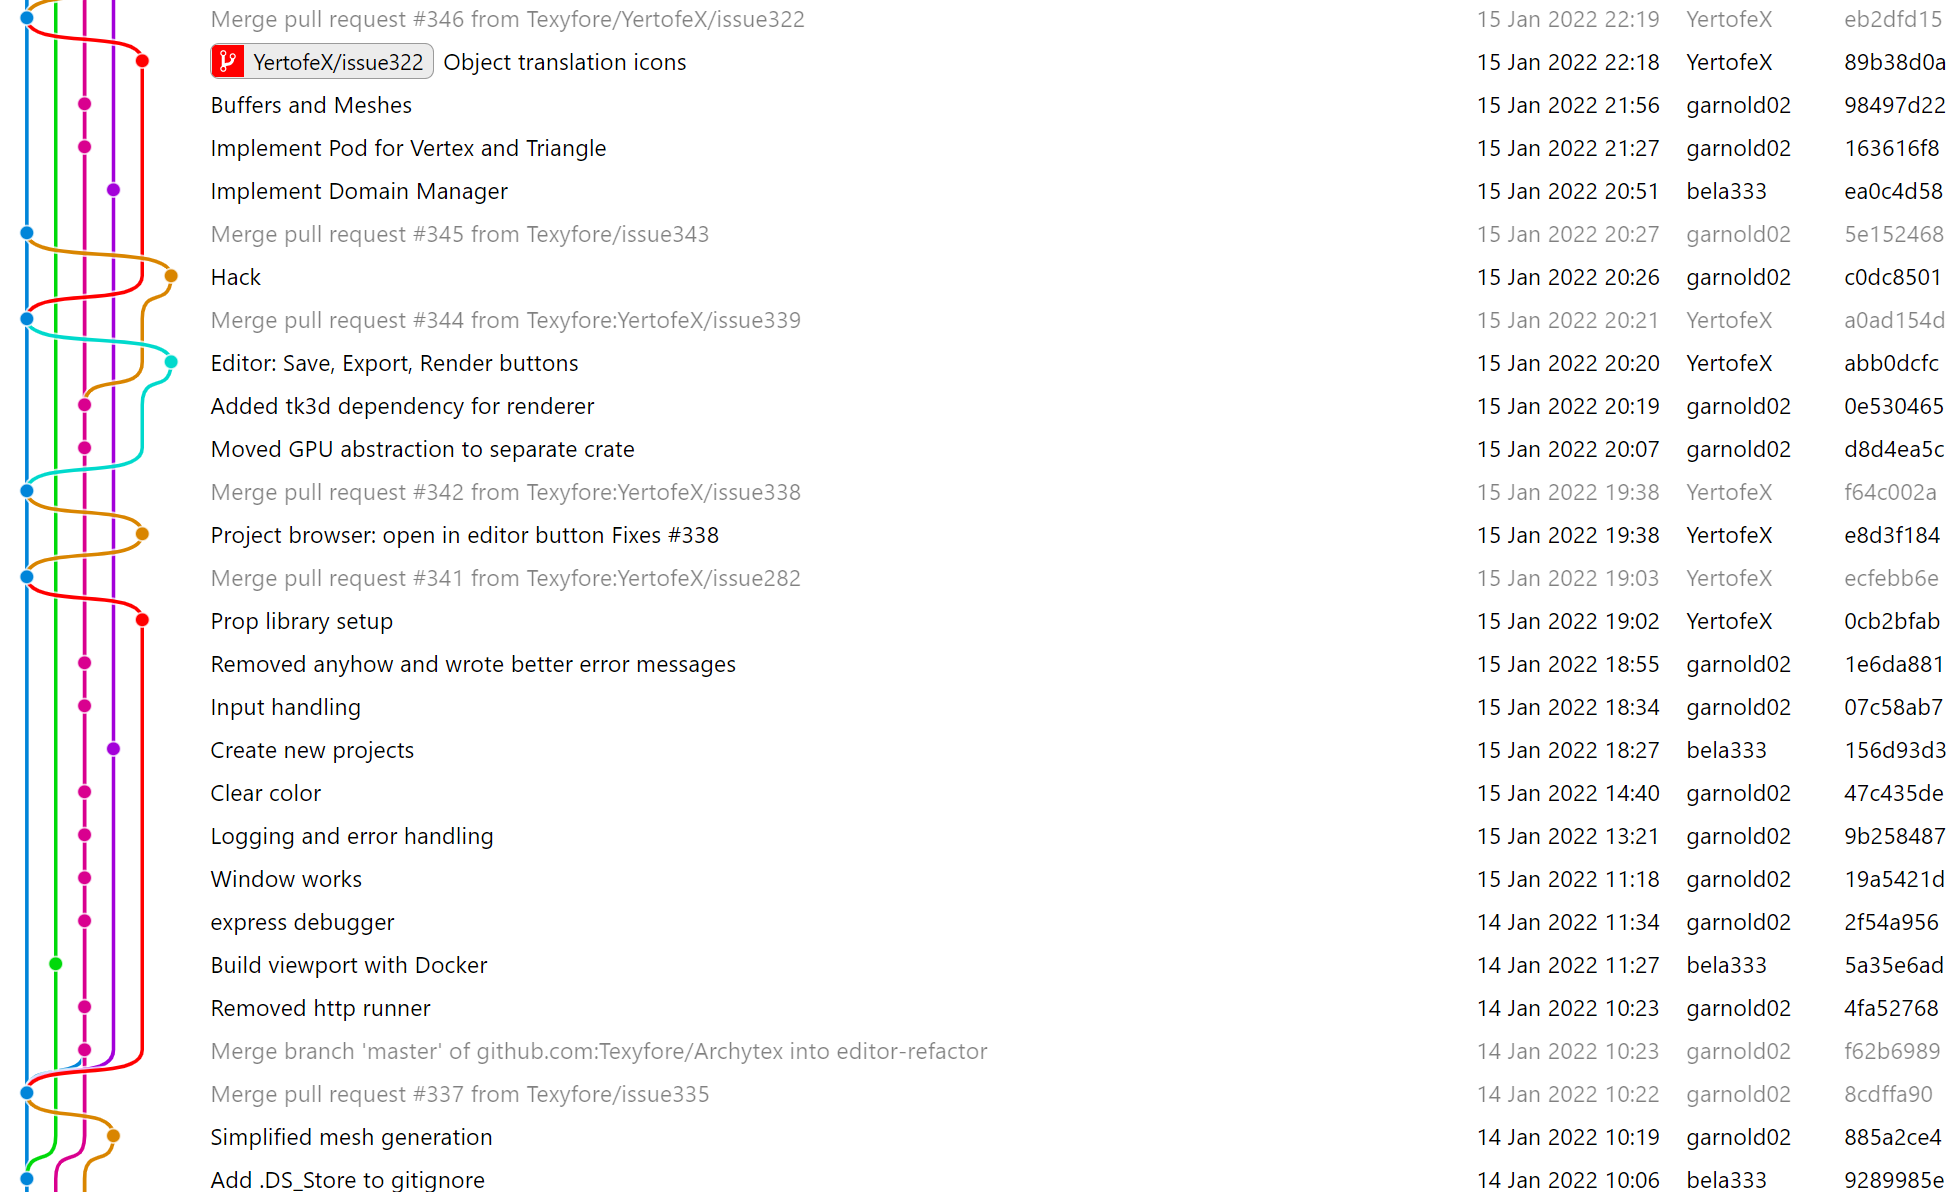
\includegraphics[width=.9\textwidth]{parts/developer-documentation/work/images/git-history.png}
  \caption{Git history képernyőkép}
\end{figure}

\subsection{GitHub használata}
Az Archytex projektet egy GitHub repository-ban fejlesztettük. Ez lehetővé tette, hogy bárhonnan, bármilyen gépről tudjuk fejleszteni az applikációt.

\begin{figure}[h]
  \centering
  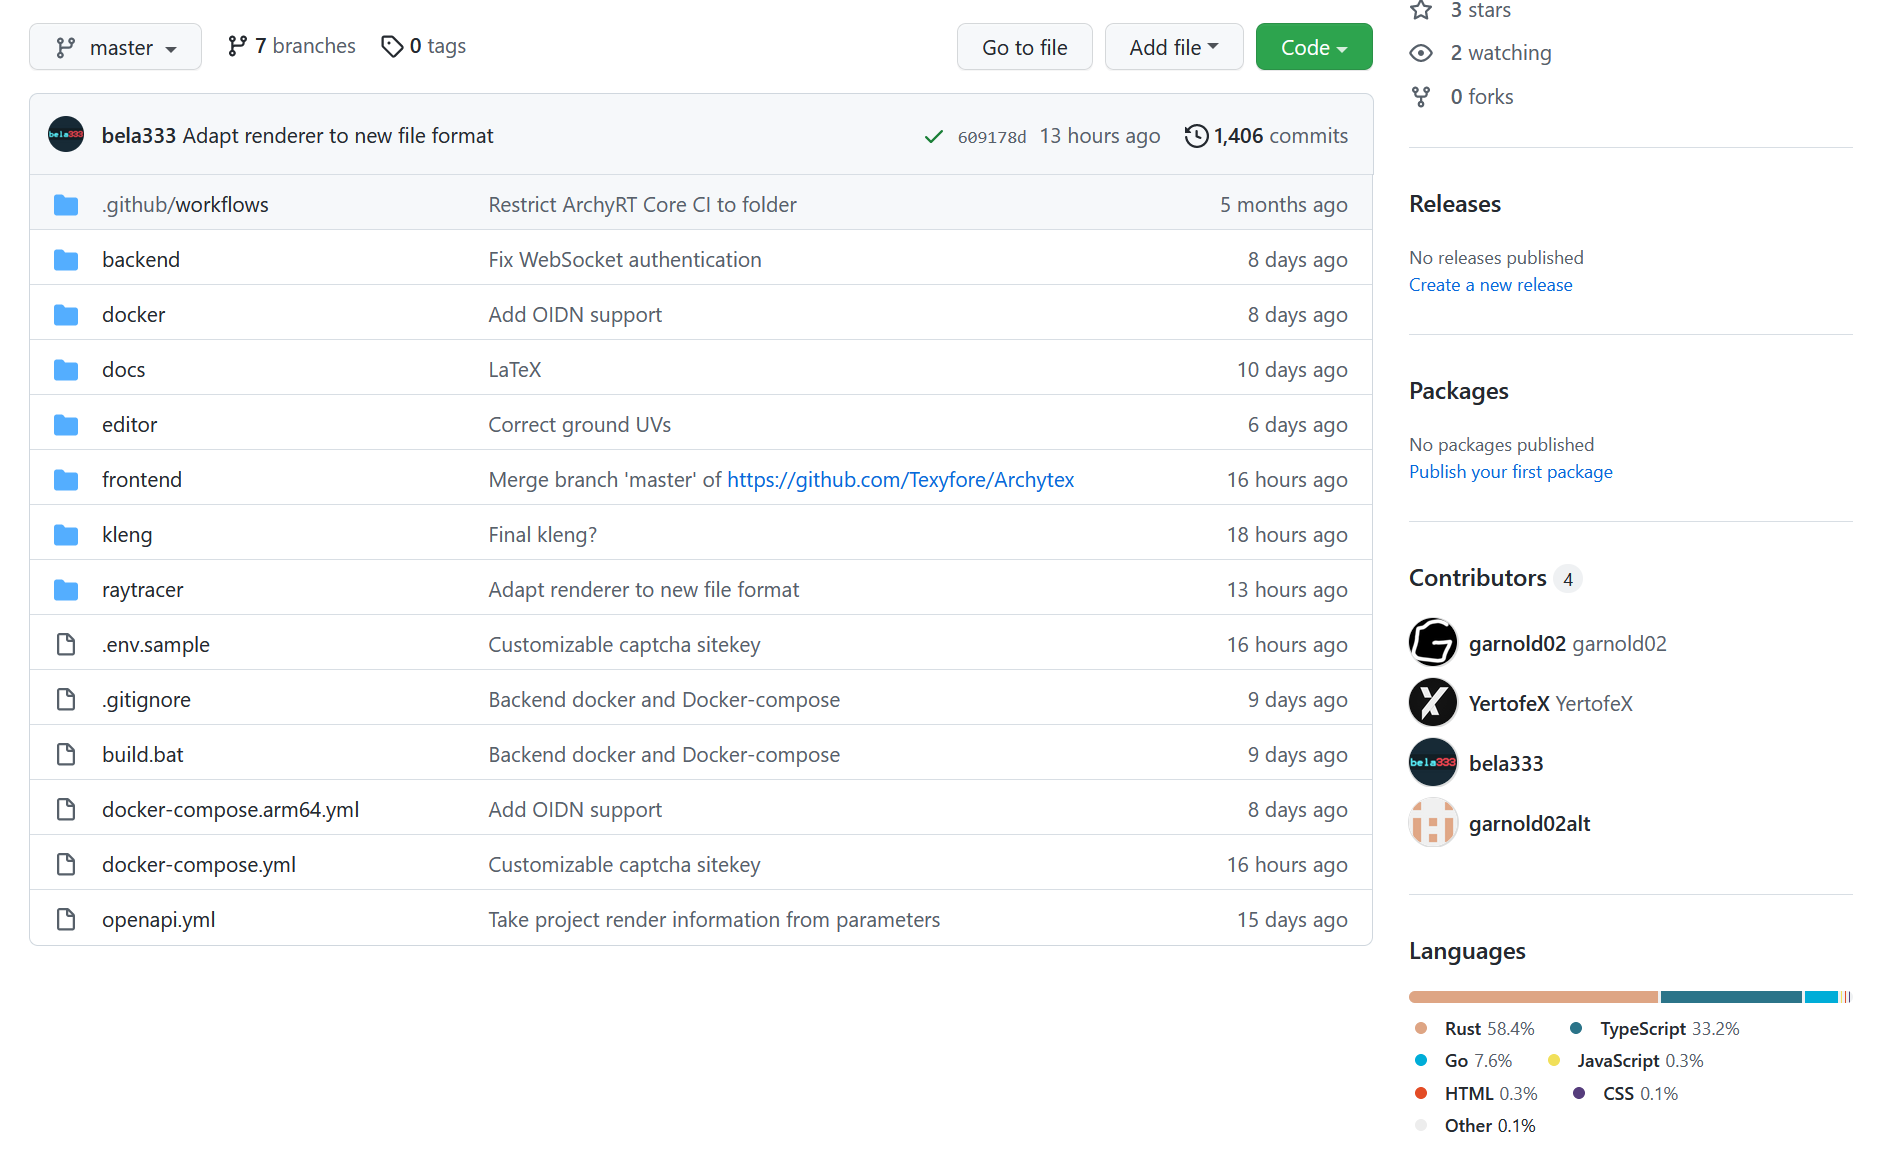
\includegraphics[width=.9\textwidth]{parts/developer-documentation/work/images/repository.png}
  \caption{Az Archytex repository képernyőképe}
\end{figure}

Hogy követni tudjuk, kinek milyen feladata van, létrehoztunk egy kanban\footnote{Kanban: 'elkészítendő', 'folyamatban' és 'elkészült' oszlopokból álló, 3 oszlopos feladattábla} típusú táblát GitHub-on, ahol az issue-kat kártyák formájában tudtuk kezelni. A kártyák kategorizálására címkéket használtunk, az ütemterv betartásának segítéséhez pedig mérföldköveket.

\begin{figure}[h]
  \centering
  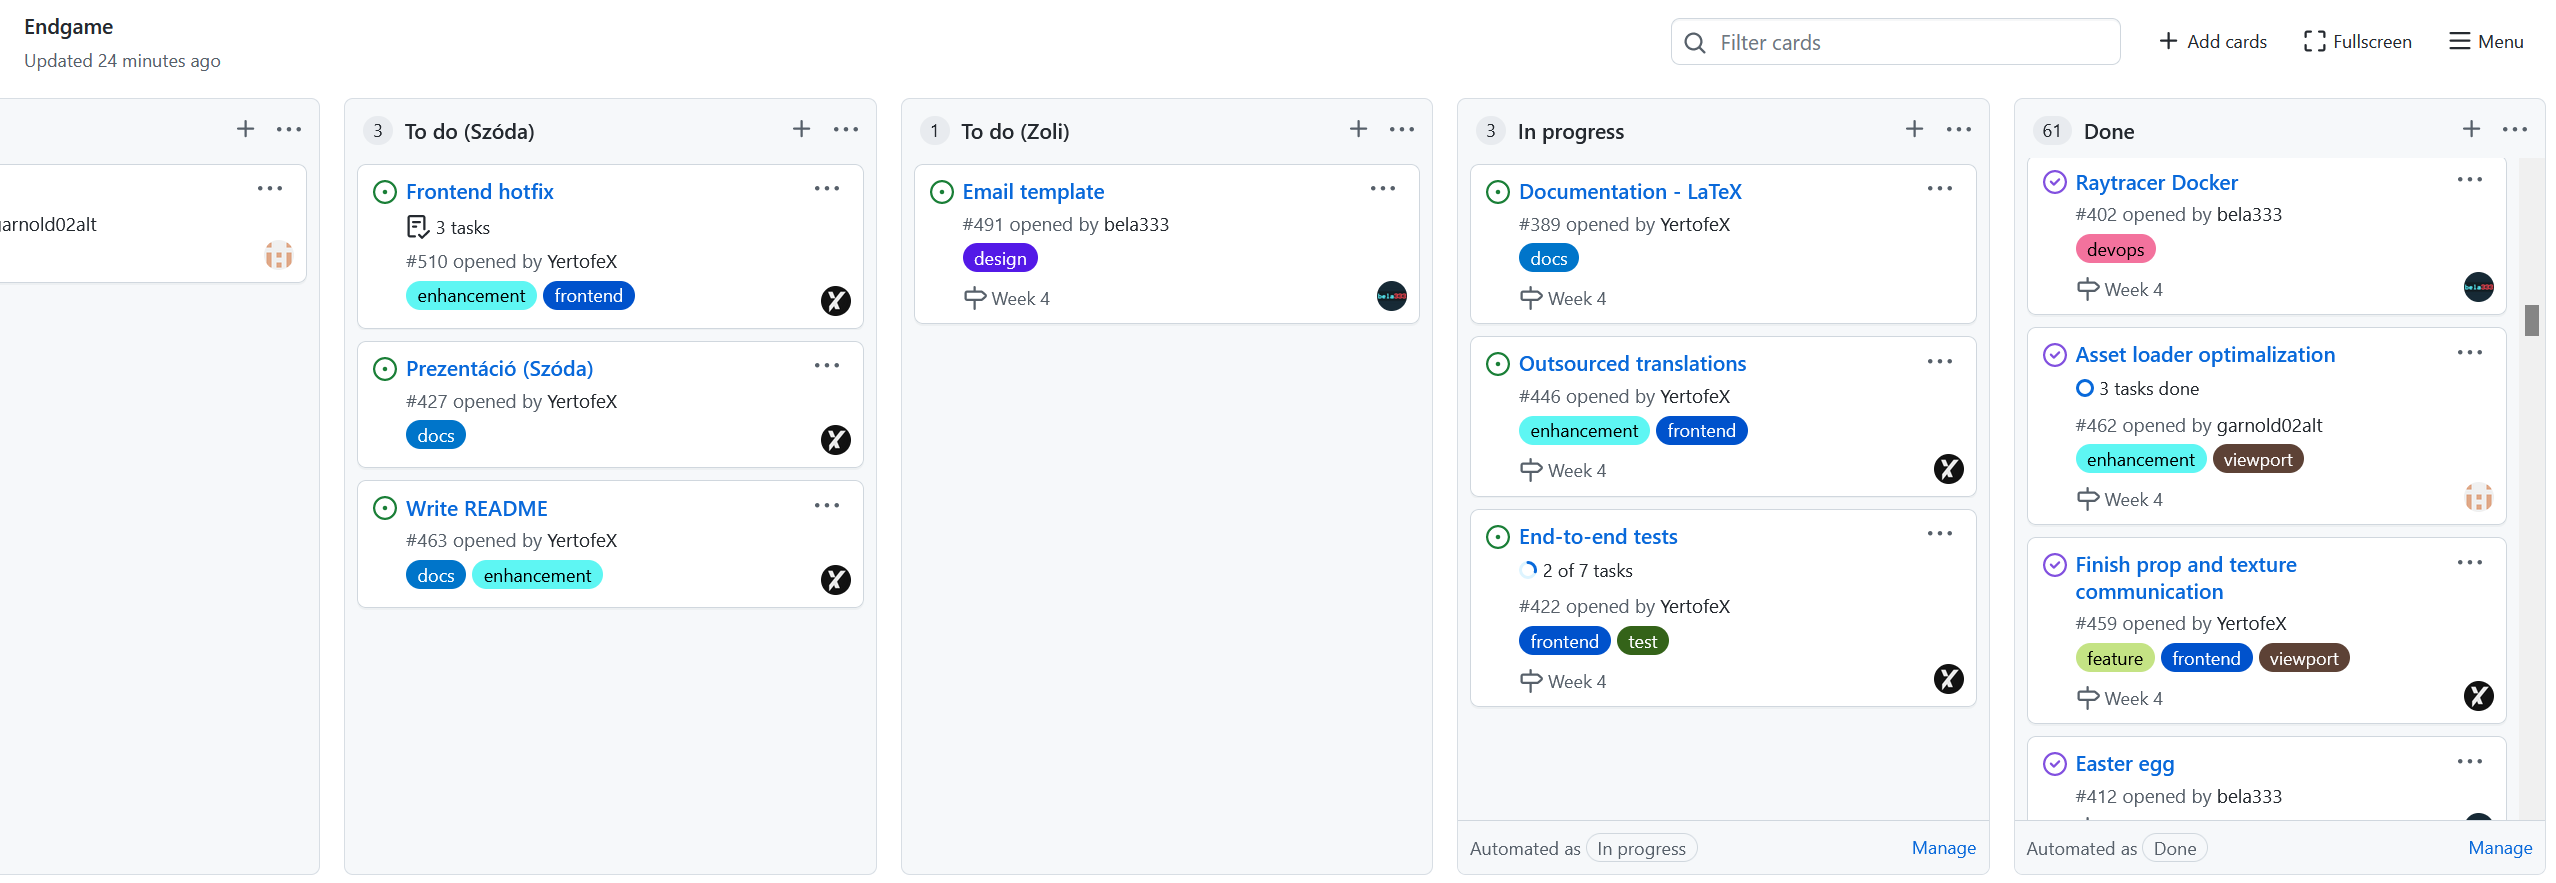
\includegraphics[width=.9\textwidth]{parts/developer-documentation/work/images/github-project.png}
  \caption{Projekt nézet az Archytex repository-ban}
\end{figure}